% Slide 8
\begin{frame}[fragile]
\frametitle{Practical Evaluation}

\begin{columns}[c]

\column{0.4\textwidth}

\begin{figure}
\vspace*{-0.5cm}
\caption{Message structure}
\vspace*{-0.85cm}
\begin{lstlisting}[language=C,frame=single,numbers=none]
typedef struct {
    (*@\texttt{\color{blue}uint8\_t}@*)  type;
    (*@\texttt{\color{blue}uint8\_t}@*)  addr_len;
    (*@\texttt{\color{blue}uint8\_t}@*)  uname_len;
    (*@\texttt{\color{blue}uint16\_t}@*) len;
    (*@\texttt{\color{blue}char}@*)    *addr;
    (*@\texttt{\color{blue}char}@*)    *uname;
} msg_t;
\end{lstlisting}
\end{figure}

\begin{figure}
\vspace*{-1cm}
\caption{Vulnerable parsing code}
\vspace*{-1cm}
\begin{lstlisting}[language=C,frame=single,numbers=none]
// UNSAFE read
memcpy(msg->addr,
       &(buf[idx]),
       msg->addr_len);
idx += msg->addr_len;
msg->addr[msg->addr_len] = '\0';
// UNSAFE read
memcpy(msg->uname,
       &(buf[idx]),
       msg->uname_len);
msg->uname[msg->uname_len] = '\0';
// UNSAFE write
memset(buf, 0, msg->len);
\end{lstlisting}
\end{figure}


\column{0.6\textwidth}

\begin{center}
\begin{figure}
\vspace*{-0.6cm}
\caption{\texttt{afl} run}
\vspace*{-0.5cm}
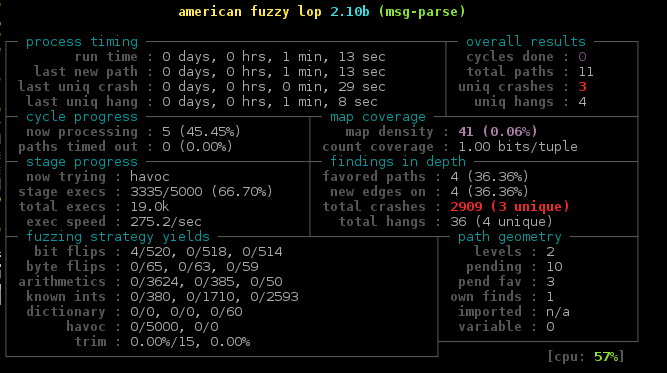
\includegraphics[scale=0.32]{../figures/afl-run}
\end{figure}
\end{center}

\begin{center}
\begin{varwidth}{0.7\textwidth}
\begin{figure}
\vspace*{-1cm}
\begin{lstlisting}[numbers=none]
01 (*@\SoulColor\hl{9c}@*) 02 00 23 6e 57 47 59 50 51 49
53 63 57 47 6c 49 35 71 6b 42 59 4b
4b 36 31 76 58 56 68 73 6f 57 68\end{lstlisting}
\caption{\texttt{afl}-generated Test Case}
\end{figure}
\end{varwidth}
\end{center}


\end{columns}


\end{frame}
